\documentclass[border=0.2cm]{standalone}

\usepackage{tikz}
\usetikzlibrary{arrows, automata, positioning}

\begin{document}

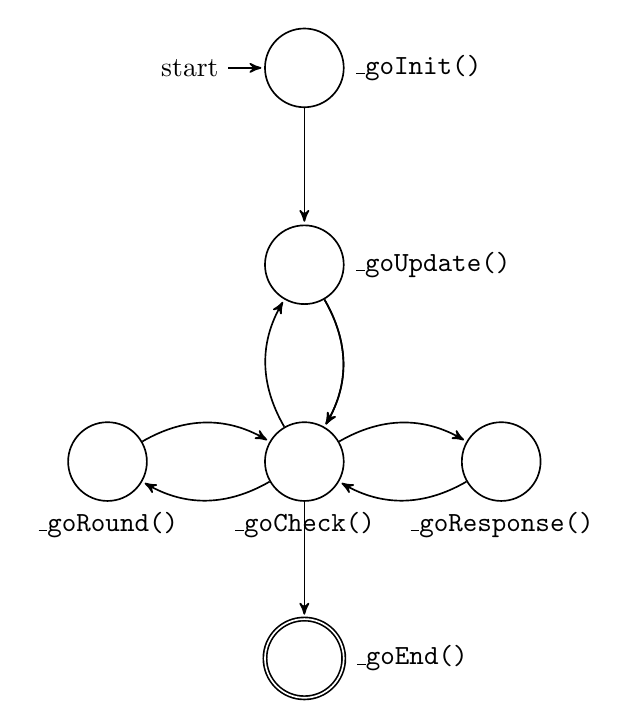
\begin{tikzpicture}[
    ->,
    >=stealth',
    shorten >=1pt,
    auto,
    node distance=2.5cm,
    semithick,
    state/.style={circle, draw, minimum size=1cm}]
]
    \tikzstyle{every state}=[fill={rgb:black,1;white,10}]

    \node[state,initial,label=right:\texttt{\_goInit()}] 	(Init)							{};
    \node[state,label=right:\texttt{\_goUpdate()}]			(Update)   	[below of=Init] 	{};
    \node[state,label=below:\texttt{\_goCheck()}]     		(Check)  	[below of=Update] 	{};
    \node[state,label=below:\texttt{\_goResponse()}]  		(Response)	[right of=Check] 	{};
    \node[state,label=below:\texttt{\_goRound()}]    		(Round)		[left of=Check] 	{};
    \node[state,accepting,label=right:\texttt{\_goEnd()}]	(End)		[below of=Check]  	{};

    \path[->]
    (Init)  	edge node				{} (Update)
    (Update) 	edge [bend left] node 	{} (Check)
    (Check) 	edge [bend left] node 	{} (Round)
                edge [bend left] node 	{} (Response)
                edge [bend left] node 	{} (Update)
                edge node 				{} (End)
    (Response)	edge [bend left] node 	{} (Check)
    (Round)		edge [bend left] node 	{} (Check)
    (Update)	edge [bend left] node 	{} (Check);
\end{tikzpicture}

\end{document}